\documentclass{article}
\usepackage[a4paper,
    left=1.8cm,
    right=1.8cm,
    top=2.2cm,
    bottom=2.2cm]{geometry}
% --- Required Packages ---
\usepackage[utf8]{inputenc}
\usepackage{amsmath}
\usepackage{amssymb}
\usepackage{longtable}
\usepackage{booktabs}
\usepackage{graphicx}
\usepackage{tabularx} % FIXED: Added missing package for tabularx
\usepackage{float}    % FIXED: Added missing package for [H] specifier

\begin{document} % FIXED: Added missing begin document command

\begin{table}[H] 
\centering 
\renewcommand{\arraystretch}{1.3} 
\begin{tabularx}{\textwidth}{|p{4cm}|X|} 
\hline 
\textbf{Experiment No.} & 2 \\ \hline 
\textbf{Experiment Title} & Email Spam/Ham Classification using Naive Bayes and
KNN \\ \hline 
\textbf{Student Name} & Sathiya Priyan \\ \hline 
\textbf{Register Number} & 3122247001058 \\ \hline 
\textbf{Faculty} & Dr. Poreddy Ajay Kumar Reddy \\ \hline 
\textbf{Submission Date} & 26-07-2026 \\ \hline 
\end{tabularx} 
\end{table} 

\section{Objective}

The objective of this experiment is to classify email messages as Spam or Ham using machine learning algorithms. The SpamBase dataset is preprocessed before model training, and Gaussian Naive Bayes, Multinomial Naive Bayes, Bernoulli Naive Bayes, and K-Nearest Neighbors (KNN) classifiers are implemented for spam classification. Finally, the models are evaluated using performance metrics to determine the most effective classifier for spam detection.

%%%%%%%%%%%%%%%%%%%%%%%%%%%%%%%%%%%%%%%%%%%%%%%%%%%%%%%%%% 
\section{Problem Statement} 
Email spam detection is a binary classification problem in machine learning. The objective of this experiment is to classify email messages as either \textbf{Spam} or \textbf{Ham (Not Spam)} using the SpamBase dataset. Different Naive Bayes classifiers and the K-Nearest Neighbors (KNN) algorithm are implemented and compared using standard performance metrics to identify the best-performing classifier. 

%%%%%%%%%%%%%%%%%%%%%%%%%%%%%%%%%%%%%%%%%%%%%%%%%%%%%%%%%% 
\section{Dataset Description} 
The SpamBase dataset is a benchmark dataset used for email spam classification. It contains numerical features extracted from email messages, such as word frequencies, character frequencies, and capital letter statistics. 

\begin{longtable}{|p{5cm}|p{9cm}|} 
\hline 
\textbf{Dataset Property} & \textbf{Description} \\ \hline 
Dataset Name & SpamBase Dataset \\ \hline 
Dataset Source & UCI Machine Learning Repository \\ \hline 
Number of Samples & 4601 email messages \\ \hline 
Number of Features & 57 input features \\ \hline 
Target Variable & class (0 = Ham, 1 = Spam) \\ \hline 
Number of Classes & 2 \\ \hline 
Missing Values & None \\ \hline 
Train-Test Split & 80\% Training, 20\% Testing \\ \hline 
\end{longtable} 

\subsection*{Dataset Overview} 
The SpamBase dataset consists of numerical features representing the frequency of specific words, special characters, and capital letters in email messages. These features are used to classify emails into two categories: Spam and Ham. Since the dataset contains no missing values, only duplicate checking and feature scaling were required before model training. 

%%%%%%%%%%%%%%%%%%%%%%%%%%%%%%%%%%%%%%%%%%%%%%%%%%%%%%%%%% 
\newpage
\section{Exploratory Data Analysis} 
Exploratory Data Analysis (EDA) was performed to understand the characteristics of the dataset before training the machine learning models. 

\subsection{Dataset Overview} 
The SpamBase dataset contains numerical attributes extracted from email messages. These attributes represent the frequency of commonly occurring words, special characters, and capital letter statistics that help distinguish spam emails from legitimate emails. 

\begin{itemize} 
\item Number of samples: 4601 
\item Number of features: 57 
\item Target variable: class 
\item Number of classes: 2 (Spam and Ham) 
\end{itemize} 

\subsection{Statistical Summary} 
The statistical summary provides information about the distribution of numerical features such as mean, standard deviation, minimum, and maximum values. Since all input attributes are numerical, descriptive statistics help understand the range and variability of the dataset. 

\subsection{Missing Value Analysis} 
The dataset contains no missing values. Therefore, no missing value imputation was required before model training. 

\subsection{Class Distribution}

The class distribution was analyzed using a count plot to determine whether the dataset contains a balanced number of spam and ham emails.

\begin{figure}[H]
\centering
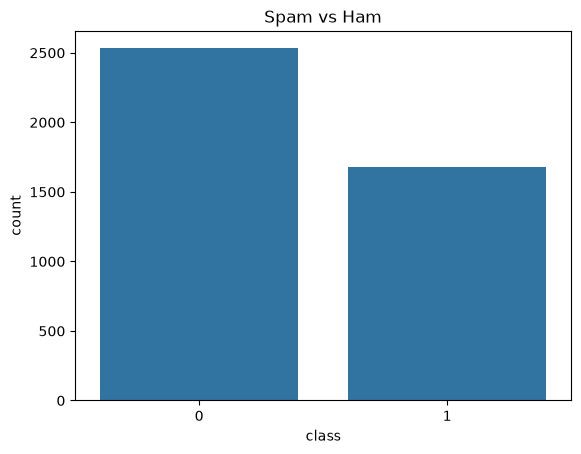
\includegraphics[width=0.6\linewidth]{class_distribution.png}
\caption{Distribution of Spam and Ham Emails}
\end{figure}

\textbf{Inference:}

\begin{itemize}
\item The dataset contains two classes: Spam and Ham.
\item Both classes are reasonably represented in the dataset.
\item The class distribution indicates that the dataset is suitable for binary classification.
\item Understanding the class distribution helps in selecting appropriate evaluation metrics.
\end{itemize} 

\subsection{Correlation Matrix}

A correlation heatmap was generated to study the relationship among numerical features in the SpamBase dataset.

\begin{figure}[H]
\centering
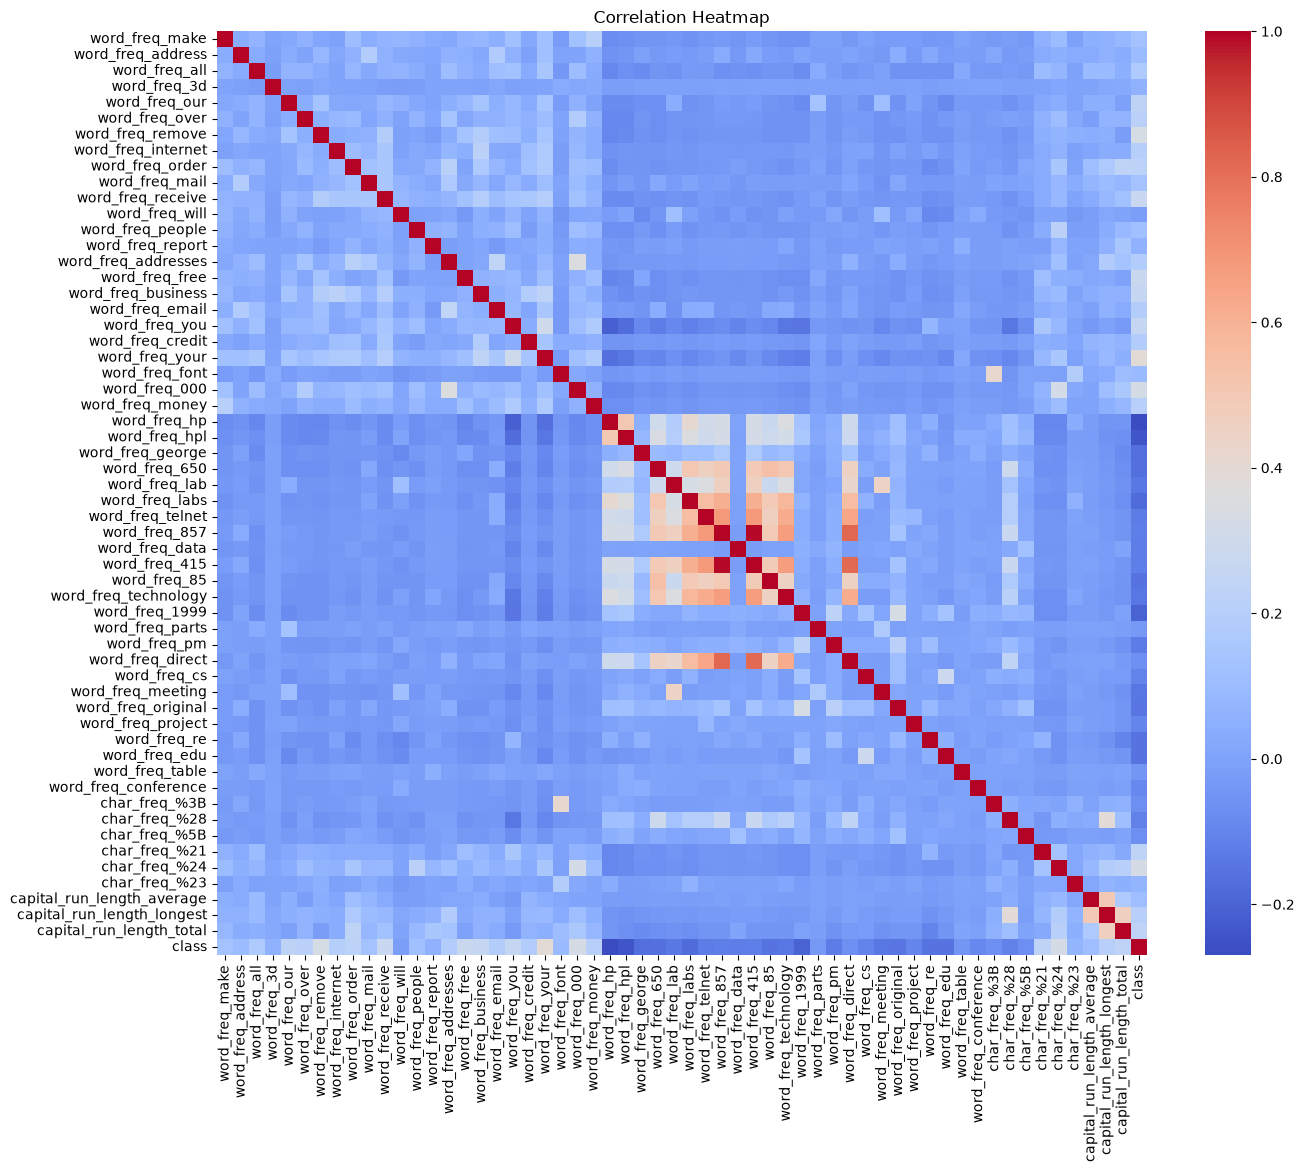
\includegraphics[width=\linewidth]{correlation_heatmap.png}
\caption{Correlation Heatmap of SpamBase Features}
\end{figure}

\textbf{Inference:}

\begin{itemize}
\item Most features exhibit low to moderate correlation with one another.
\item No severe multicollinearity is observed among the input features.
\item Some word-frequency features show positive correlation with the target class.
\item The correlation matrix helps understand feature relationships before model training.
\end{itemize}

\subsection{Feature Distribution}

Histograms and box plots were used to visualize the distribution of feature values and identify possible outliers.

\begin{figure}[H]
\centering
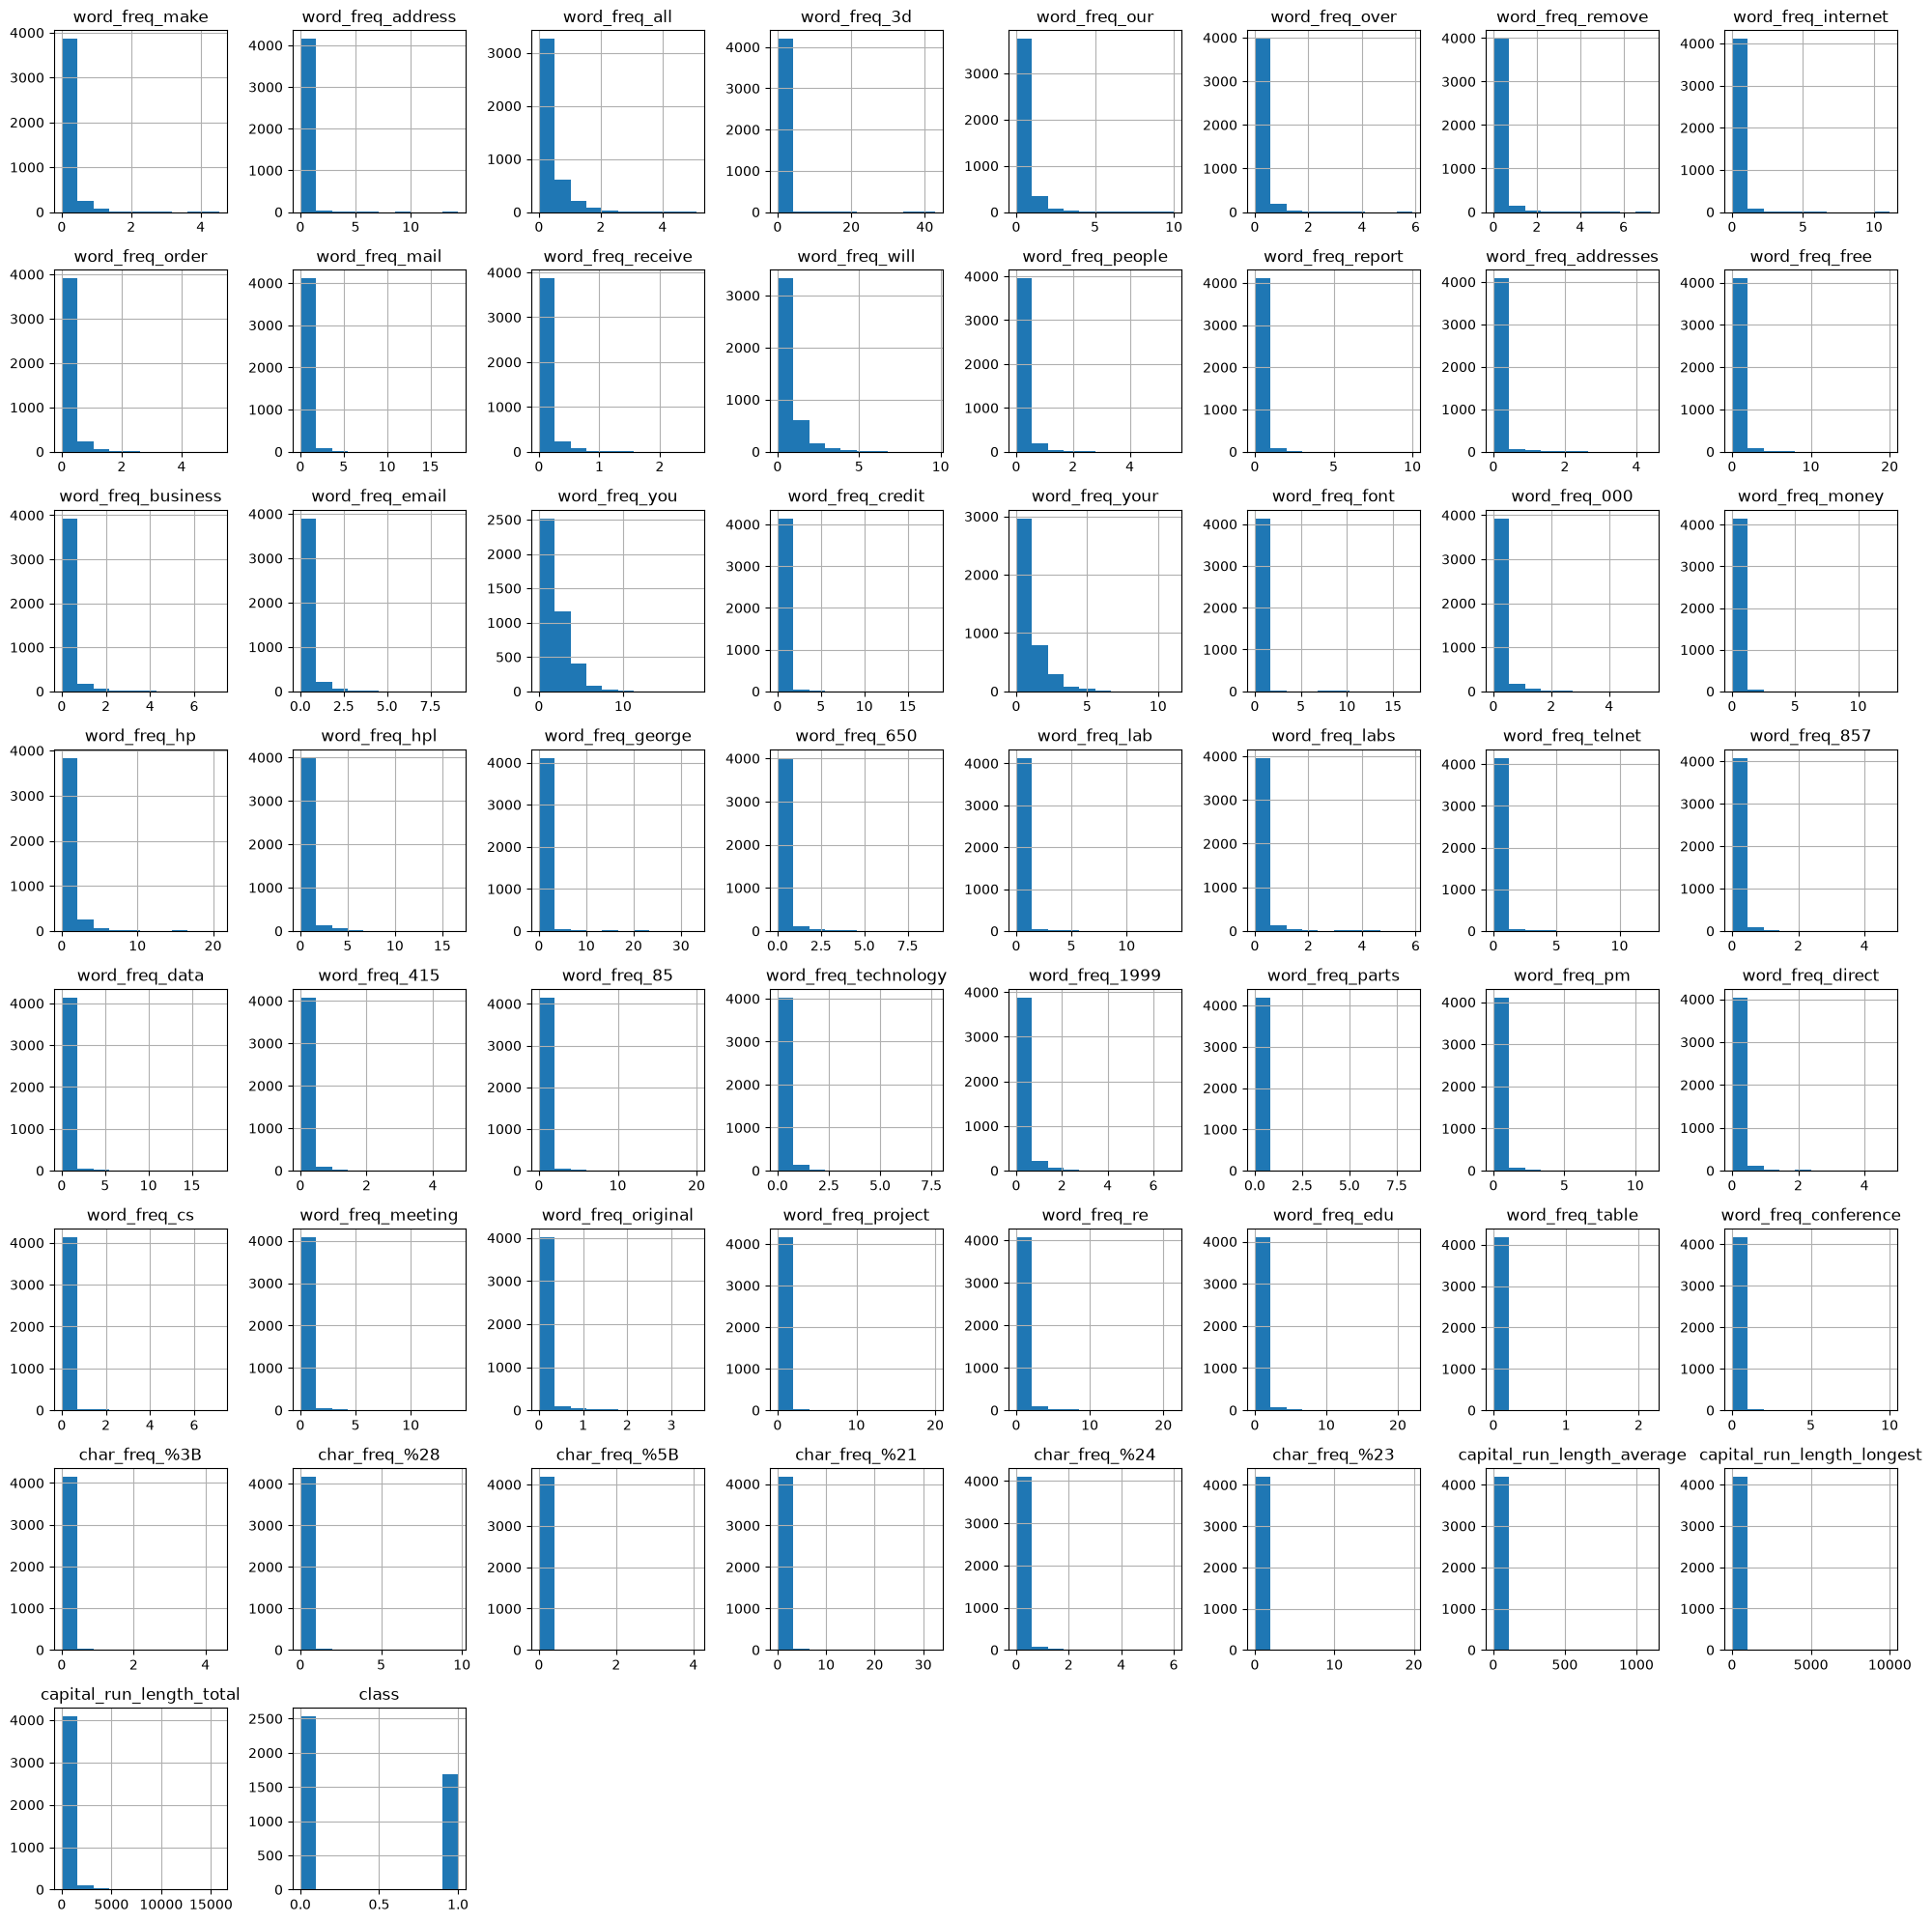
\includegraphics[width=\linewidth]{feature_histograms.png}
\caption{Distribution of Features}
\end{figure}

\begin{figure}[H]
\centering
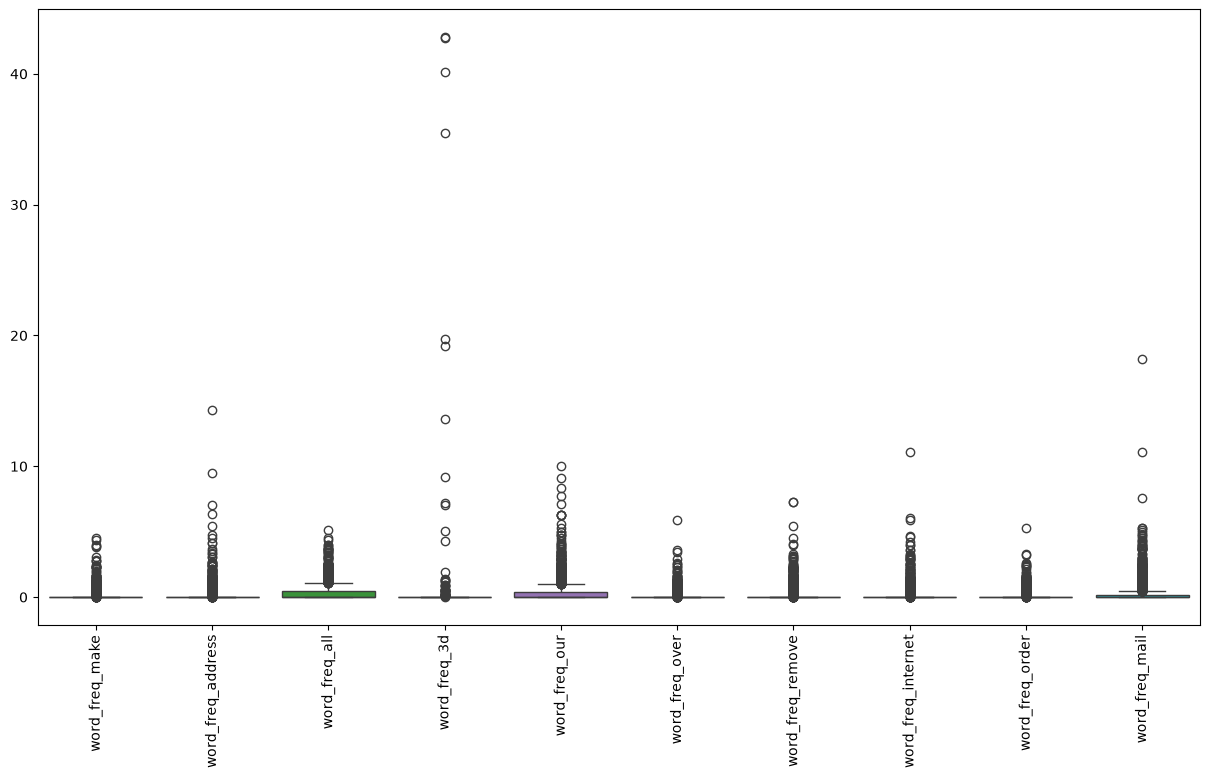
\includegraphics[width=\linewidth]{boxplot_features.png}
\caption{Box Plot of Selected Features}
\end{figure}

\textbf{Inference:}

\begin{itemize}
\item Most features are positively skewed.
\item Several attributes contain outliers, which are common in email frequency data.
\item Feature scaling is beneficial because the attributes have different ranges.
\item The distributions justify the preprocessing performed before model training.
\end{itemize} 

%%%%%%%%%%%%%%%%%%%%%%%%%%%%%%%%%%%%%%%%%%%%%%%%%%%%%%%%%% 




\newpage
\section{Data Preprocessing}

The SpamBase dataset was preprocessed before training the machine learning models. The preprocessing steps performed are described below.

\subsection*{Missing Value Handling}

The dataset was checked for missing values using the \texttt{isnull()} function. No missing values were found in any of the 58 attributes; therefore, no imputation or data cleaning was required.

\subsection*{Encoding}

The SpamBase dataset consists entirely of numerical features representing word frequencies, character frequencies, and capital letter statistics. Since all input features were already in numerical format, no categorical encoding techniques such as Label Encoding or One-Hot Encoding were required.

\subsection*{Feature Scaling}

Different feature scaling techniques were applied based on the requirements of each classification algorithm.

\begin{itemize}
    \item \textbf{StandardScaler} was applied before training the Gaussian Naive Bayes and K-Nearest Neighbors (KNN) classifiers.
    \item \textbf{MinMaxScaler} was used for the Multinomial Naive Bayes classifier to transform feature values into the range of 0 to 1.
    \item \textbf{Binarizer} was applied before training the Bernoulli Naive Bayes classifier to convert numerical feature values into binary values.
\end{itemize}

\subsection*{Train-Test Split}

The dataset was divided into training and testing sets using an 80:20 ratio. Stratified sampling was employed to preserve the class distribution in both the training and testing datasets.

\subsection*{Feature Engineering}

No additional feature engineering techniques were applied. The original numerical features extracted from the SpamBase dataset were used directly for model training after the required preprocessing steps.

\section{Machine Learning Algorithms}

The experiment implements three variants of the Naive Bayes classifier and the K-Nearest Neighbors (KNN) classifier for email spam detection.

\subsection{Gaussian Naive Bayes}

\textbf{Working Principle}

Gaussian Naive Bayes assumes that all features follow a Gaussian (Normal) distribution and that every feature is conditionally independent given the class label.

\textbf{Mathematical Formulation}

\[
P(C|X)=\frac{P(X|C)P(C)}{P(X)}
\]

where \(C\) represents the class and \(X\) represents the feature vector.

\textbf{Advantages}

\begin{itemize}
\item Simple and computationally efficient.
\item Performs well on high-dimensional datasets.
\item Requires relatively small training data.
\end{itemize}

\textbf{Limitations}

\begin{itemize}
\item Assumes feature independence.
\item Assumes Gaussian distribution of features.
\item Performance decreases if assumptions are violated.
\end{itemize}

\subsection{Multinomial Naive Bayes}

\textbf{Working Principle}

Multinomial Naive Bayes is designed for count or frequency data. It estimates the probability of each class using the frequency of features.

\textbf{Mathematical Formulation}

\[
P(C|X)\propto P(C)\prod_{i=1}^{n}P(x_i|C)
\]

\textbf{Advantages}

\begin{itemize}
\item Suitable for text classification.
\item Fast training and prediction.
\item Works well with word-frequency features.
\end{itemize}

\textbf{Limitations}

\begin{itemize}
\item Requires non-negative feature values.
\item Assumes feature independence.
\item Sensitive to feature distribution.
\end{itemize}

\subsection{Bernoulli Naive Bayes}

\textbf{Working Principle}

Bernoulli Naive Bayes works with binary features by considering whether a feature is present or absent.

\textbf{Mathematical Formulation}

\[
P(C|X)\propto P(C)\prod_{i=1}^{n}P(x_i|C)
\]

where each feature takes either 0 or 1.

\textbf{Advantages}

\begin{itemize}
\item Effective for binary features.
\item Fast and memory efficient.
\item Performs well for text classification.
\end{itemize}

\textbf{Limitations}

\begin{itemize}
\item Requires binary input.
\item May lose information after binarization.
\item Assumes feature independence.
\end{itemize}

\subsection{K-Nearest Neighbors (KNN)}

\textbf{Working Principle}

KNN is a non-parametric supervised learning algorithm that classifies a sample based on the majority class of its nearest neighbours.

\textbf{Mathematical Formulation}

Euclidean Distance:

\[
d(x,y)=\sqrt{\sum_{i=1}^{n}(x_i-y_i)^2}
\]

Manhattan Distance:

\[
d(x,y)=\sum_{i=1}^{n}|x_i-y_i|
\]

\textbf{Advantages}

\begin{itemize}
\item Simple and easy to implement.
\item No explicit training phase.
\item Effective for non-linear decision boundaries.
\end{itemize}

\textbf{Limitations}

\begin{itemize}
\item Computationally expensive during prediction.
\item Sensitive to feature scaling.
\item Performance depends on the choice of \(k\).
\end{itemize}

\section{Experimental Setup}

\begin{table}[H]
\centering
\begin{tabular}{ll}
\toprule
Python Version & 3.x \\
Scikit-Learn Version & Latest installed version \\
IDE & Jupyter Notebook \\
Operating System & Windows 11 \\
Hardware & Intel Core Ultra 7 Processor, 32 GB RAM \\
\bottomrule
\end{tabular}
\end{table}
\section{Hyperparameter Selection}

\begin{table}[H]
\centering
\begin{tabular}{ll}
\toprule
Parameter & Value\\
\midrule
n\_neighbors & 9\\
Weights & distance\\
Metric & manhattan\\
Algorithm & auto\\
Cross Validation & 5-fold\\
Best CV Accuracy & 0.9139\\
\bottomrule
\end{tabular}
\caption{Best Parameters Obtained Using GridSearchCV}
\end{table}

\section{Results}

\begin{table}[H]
\centering
\begin{tabular}{lc}
\toprule
Metric & Value\\
\midrule
Accuracy & 0.9276\\
Precision & 0.9148\\
Recall & 0.8631\\
F1-score & 0.8882\\
ROC-AUC & 0.9546\\
\bottomrule
\end{tabular}
\caption{Performance of the Best KNN Classifier}
\end{table}

\section{Result Visualization}

\subsection{Correlation Matrix}

\begin{figure}[H]
\centering
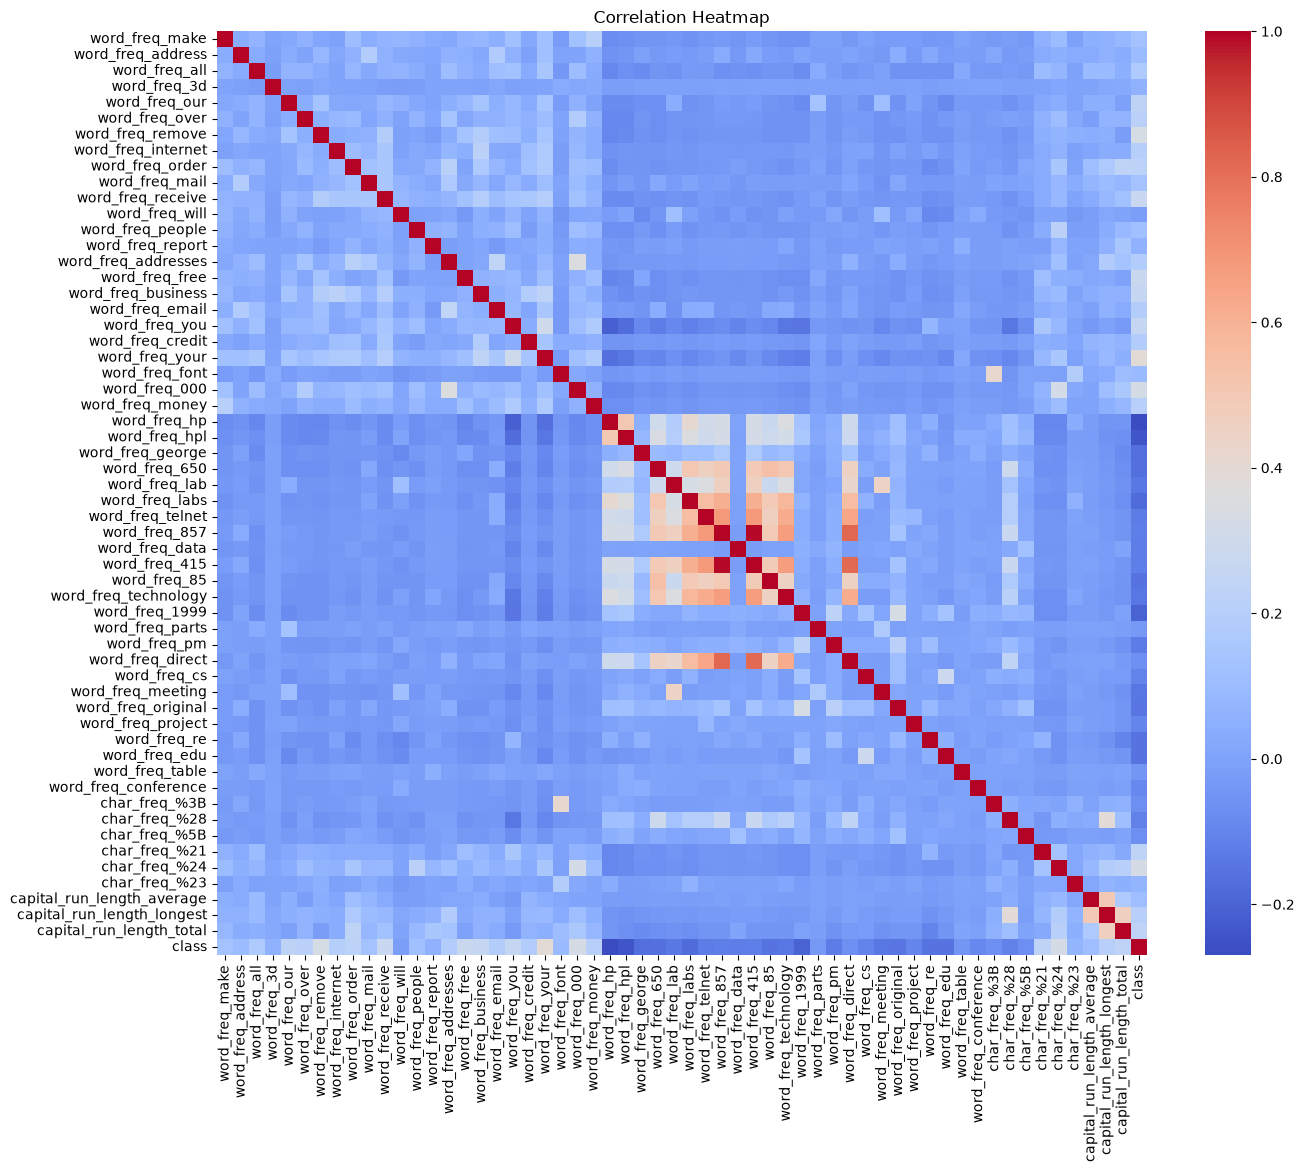
\includegraphics[width=0.8\linewidth]{correlation_heatmap.png}
\caption{Correlation Matrix of SpamBase Features}
\end{figure}

\textbf{Inference:}
\begin{itemize}
    \item The correlation matrix shows the relationship among numerical features.
    \item Most features exhibit weak to moderate correlation.
    \item No severe multicollinearity is observed among the input features.
    \item The heatmap helps understand feature relationships before model training.
\end{itemize}

%%%%%%%%%%%%%%%%%%%%%%%%%%%%%%%%%%%%%%%%%%%%%%%%%%%%%%%%%%%%

\subsection{Class Distribution}

\begin{figure}[H]
\centering
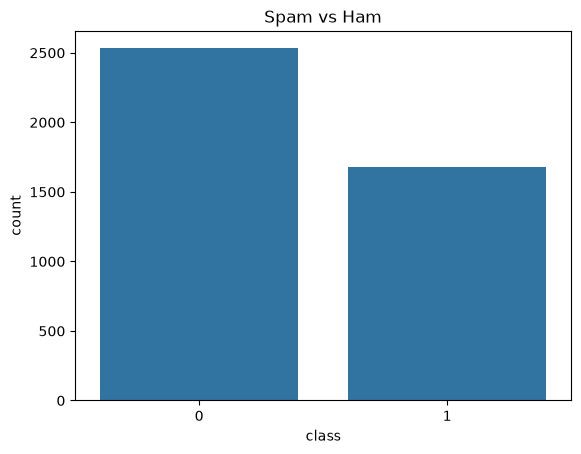
\includegraphics[width=0.6\linewidth]{class_distribution.png}
\caption{Distribution of Spam and Ham Emails}
\end{figure}

\textbf{Inference:}
\begin{itemize}
    \item The dataset contains two classes: Spam and Ham.
    \item Both classes are well represented in the dataset.
    \item The class distribution is suitable for binary classification.
    \item Understanding the class balance helps evaluate classifier performance.
\end{itemize}

%%%%%%%%%%%%%%%%%%%%%%%%%%%%%%%%%%%%%%%%%%%%%%%%%%%%%%%%%%%%

\subsection{Confusion Matrix}

\begin{figure}[H]
\centering
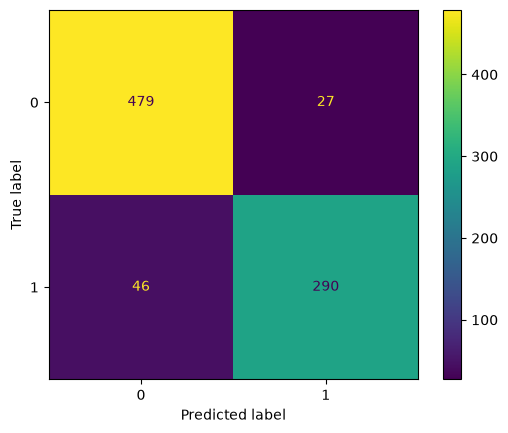
\includegraphics[width=0.6\linewidth]{confusion_matrix.png}
\caption{Confusion Matrix of the Best KNN Classifier}
\end{figure}

\textbf{Inference:}
\begin{itemize}
    \item Most spam and ham emails are correctly classified.
    \item Only a small number of false positives and false negatives are observed.
    \item The confusion matrix indicates good classification performance.
    \item The classifier effectively distinguishes spam from legitimate emails.
\end{itemize}

%%%%%%%%%%%%%%%%%%%%%%%%%%%%%%%%%%%%%%%%%%%%%%%%%%%%%%%%%%%%

\subsection{ROC Curve}

\begin{figure}[H]
\centering
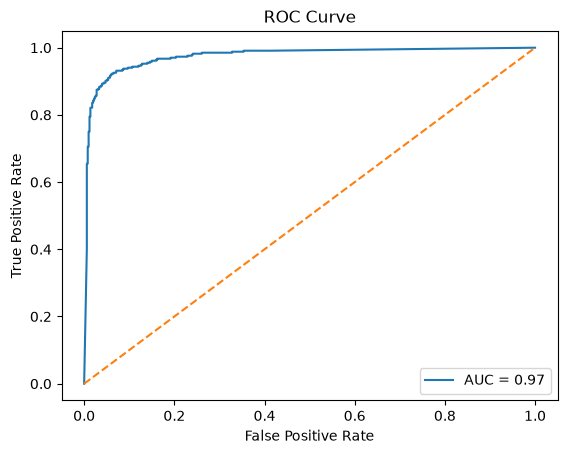
\includegraphics[width=0.7\linewidth]{roc_curve.png}
\caption{Receiver Operating Characteristic (ROC) Curve}
\end{figure}

\textbf{Inference:}
\begin{itemize}
    \item The ROC curve lies close to the upper-left corner.
    \item The classifier achieves a high ROC-AUC score.
    \item A high ROC-AUC indicates excellent discrimination between spam and ham emails.
    \item The model performs well across different classification thresholds.
\end{itemize}

%%%%%%%%%%%%%%%%%%%%%%%%%%%%%%%%%%%%%%%%%%%%%%%%%%%%%%%%%%%%

\subsection{Precision--Recall Curve}

\begin{figure}[H]
\centering
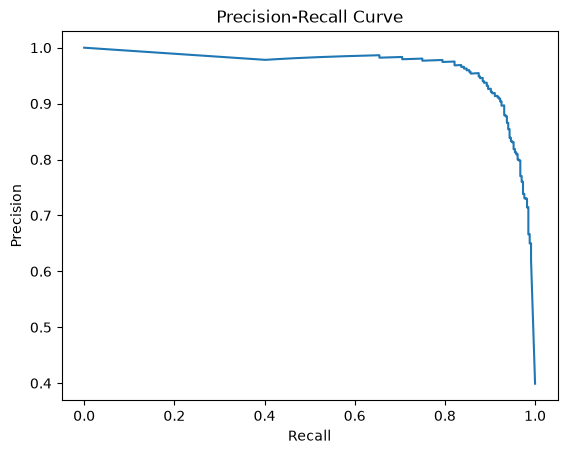
\includegraphics[width=0.7\linewidth]{precision_recall_curve.png}
\caption{Precision--Recall Curve}
\end{figure}

\textbf{Inference:}
\begin{itemize}
    \item The Precision--Recall curve demonstrates a good balance between precision and recall.
    \item Precision remains high across most recall values.
    \item The classifier maintains good performance on the positive (spam) class.
    \item This curve is especially useful for evaluating binary classification models.
\end{itemize}

%%%%%%%%%%%%%%%%%%%%%%%%%%%%%%%%%%%%%%%%%%%%%%%%%%%%%%%%%%%%

\subsection{Accuracy vs. K}

\begin{figure}[H]
\centering
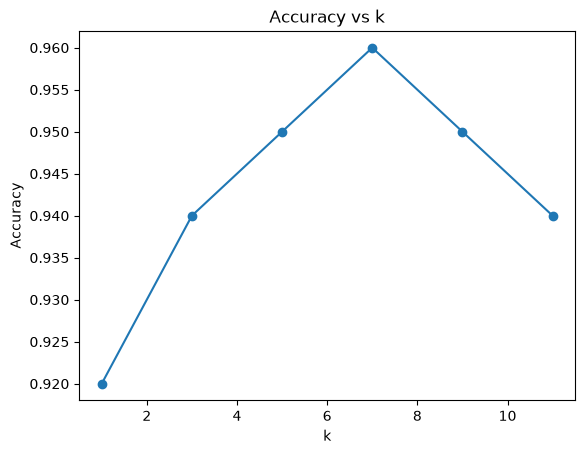
\includegraphics[width=0.7\linewidth]{accuracy_vs_k.png}
\caption{Accuracy for Different Values of K}
\end{figure}

\textbf{Inference:}
\begin{itemize}
    \item Classification accuracy varies with different values of $k$.
    \item Selecting an appropriate value of $k$ improves prediction performance.
    \item GridSearchCV identified the optimal value of $k$.
    \item This graph highlights the importance of hyperparameter tuning.
\end{itemize}

%%%%%%%%%%%%%%%%%%%%%%%%%%%%%%%%%%%%%%%%%%%%%%%%%%%%%%%%%%%%

\subsection{Classifier Comparison}

\begin{figure}[H]
\centering
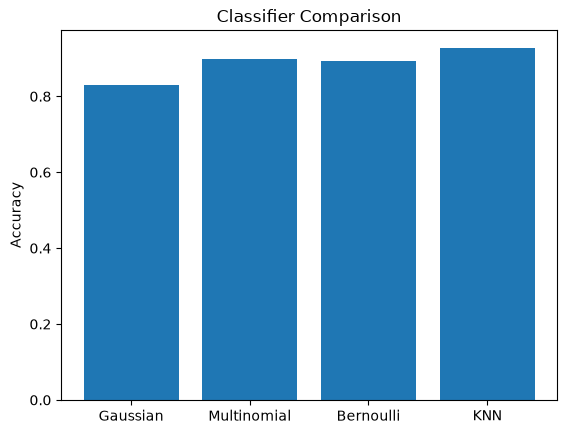
\includegraphics[width=0.7\linewidth]{classifier_comparison.png}
\caption{Comparison of Classification Algorithms}
\end{figure}

\textbf{Inference:}
\begin{itemize}
    \item K-Nearest Neighbors (KNN) achieved the highest classification accuracy.
    \item Bernoulli Naive Bayes and Multinomial Naive Bayes also produced good results.
    \item Gaussian Naive Bayes showed comparatively lower performance.
    \item Overall, the tuned KNN classifier was the best-performing model in this experiment.
\end{itemize}

\section{Discussion}

Four classification algorithms were implemented and evaluated for spam email detection. Among the Naive Bayes classifiers, Bernoulli Naive Bayes achieved better performance than Gaussian and Multinomial Naive Bayes. Hyperparameter tuning using GridSearchCV improved the performance of the KNN classifier, resulting in the highest classification accuracy.
\section{Conclusion}

The SpamBase dataset was successfully used to classify emails as Spam or Ham using Naive Bayes and K-Nearest Neighbors classifiers. Appropriate preprocessing techniques, including feature scaling and train-test splitting, were performed before model training.

\section{References}

\begin{enumerate}
\item A. Géron, \textit{Hands-On Machine Learning with Scikit-Learn, Keras and TensorFlow}, 3rd ed., O'Reilly Media, 2022.

\item C. M. Bishop, \textit{Pattern Recognition and Machine Learning}. Springer, 2006.

\item T. Hastie, R. Tibshirani and J. Friedman, \textit{The Elements of Statistical Learning}. Springer, 2009.

\item Scikit-learn Documentation. \texttt{https://scikit-learn.org}


\end{enumerate}


\end{document}
